% !TEX root = ../main.tex

\chapter{Data-driven strategies for robust forecast of continuous glucose monitoring time-series} \label{chap:diabete}
% EMBC

\begin{displayquote}
\textit{Over the past decade, continuous glucose monitoring (CGM) has proven to be a very resourceful tool for diabetes management. To date, CGM devices are employed for both retrospective and online applications. Their use allows to better describe the patients' pathology as well as to achieve a better control  of  patients' level of glycemia. The analysis of CGM sensor data makes possible to observe a wide range of metrics, such as the glycemic variability during the day or the amount of time spent below or above certain glycemic thresholds. However, due to the high variability of the glycemic signals among sensors and individuals, CGM data analysis is a non-trivial task. Standard signal filtering solutions fall short when an appropriate model personalization is not applied. State of the art data-driven strategies for online CGM forecasting rely upon the use of recursive filters. Each time a new sample is collected, such models need to adjust their parameters in order to predict the next glycemic level. In this chapter we will see that the problem of online CGM forecasting can be successfully tackled by personalized machine learning models, that do not need to recursively update their parameters.}
\end{displayquote}

\section{Introduction: modern diabetes care}
Diabetes is a chronic metabolic disorder affecting nearly $400$ million of individuals worldwide. The number of diabetic patients is increasing and it is expected to reach almost $600$ million in the next future~\cite{guariguata2014global}.
%In the world people with type 2 diabetes are $400$ million and this  number will rise to $600$ million in $2035$~\cite{guariguata2014global}. 
%http://www.who.int/diabetes/global-report/en/
%https://www.cdc.gov/diabetes/statistics/incidence/fig2.htm
According to the {\em World Health Organization}~\cite{world2016global}, the global prevalence of diabetes among adults has nearly doubled in the last few decades, rising from $4.7\%$ in 1980 to $8.5\%$ in 2014.
%and its incidence per year is $6.9$ per $1,000$ individuals~\cite{}.
%In the western population the  prevalence of diabetes is $6$ to $10\%$ .
%The incidence of diabetes type $2$ is $5-7/1000/$year \todo{non sono sicuro di aver capito}.
If not treated correctly, diabetes may cause several permanent complications, such as visual impairment and kidney failure. 
%, that heavily affect the quality of life of the patients

Hypoglycemia is a severe risk in diabetes therapy. 
The mean incidence of hypoglycemia in patients with type $1$ diabetes (T1D) 
is 1-2 events per week, while severe hypoglicemia occurs 0.1-1.5 episodes per year~\cite{van2016continuous}. 
Moreover, hypoglycemia interferes with the quality of life and increases the risks of cardiovascular events in type $2$ diabetes (T2D) patients~\cite{van2016continuous}. On the other hand, hyperglycemia associates with an increased risk of diabetes complication as well.


The most common glucose monitoring solutions are self blood glucose meters and Continuous Glucose Monitoring systems (\ac{CGM}). 
CGM devices are minimally-invasive, and can be used in daily life for retrospective or online applications~\cite{vigersky2017role}. 
CGM systems measure interstitial glucose concentration at fixed time intervals, enabling an accurate observation of glycemic variability during the day as well as the ratio of time spent in hypo/hyperglycemia. 
When CGM is employed online, an improvement of the therapy can be achieved by embedding in the system a tool that foresees glucose levels using suitable time-series models trained on past  CGM  data~\cite{sparacino2007glucose}. In this case, alarms can be generated when the glucose concentration exceeds the normal range~\cite{vigersky2017role}.
%thresholds

%Such tools implement algorithms to foresee hypo/hyperglycemic  events that can be obtained  by  generating alerts on  the basis of future glucose level forecast by  using  past  CGM  data  and  suitable time-series  models \cite{sparacino2007glucose}.
%\cite{monnier2016near}
%\todo{
%State-of-the-art in diabetes monitoring is glycemia self assessment via glucose meters~\cite{monnier2016near} NON SONO SICURO DELLA REF},   it is possible to self-manage diabetes with continuous glucose monitoring (CGM) devices. CGM systems measure interstitial glucose concentration at fixed time intervals (e.g., each $5$ minutes). 
%
%CGM enables the observation of glycemic variability during the day as well as the ratio of time spent in hypo/hyperglycemia. 
%
%
%These devices are minimally-invasive, and can be used in daily life, but, to date, they are mainly used for retrospective and online applications~\cite{vigersky2017role}. 
%
%In both cases, CGM enables the observation of glycemic variability during the day as well as the ratio of time spent in hypo/hyperglycemia. 
%
%When CGM is employed online, an improvement of the therapy can be achieved by embedding in the system a tool able to generate alerts when the glucose concentration exceeds the normal range thresholds~\cite{vigersky2017role}, based on past  CGM  data  and  suitable time-series  models \cite{sparacino2007glucose}.

%In many clinical situations


To model patient-specific Glood Glucose (BG) levels, several approaches integrating various information were proposed~\cite{bunescu2013blood, zecchin2011new}. However, the problem of glycemic level prediction is still challenging, due to the high CGM signal variability among patients and acquisition devices.

This chapter describes the third, and last, biomedical data science challenge of the Thesis. We will assume that CGM signals have structural information on time-changes of BG concentration \cite{sparacino2007glucose, bunescu2013blood} and we perform glycemic level forecasting exploring the performance of a set of purely data-driven techniques for time-series analysis.

Data-driven forecasting approaches, as opposed to models driven by an \textit{a-priori} description of the underlying phenomena, are capable of modeling input/output relationships without requiring prior knowledge on the field of use. This family of approaches can be successfully employed to obtain reliable predictions without modeling complex, and possibly not completely understood, environments. Data-driven forecasting models are widely applied in  real-world scenarios often employing a moving-window paradigm, \ie the system keeps track of the last $w$ acquisitions using them to forecast future values.

In this chapter, we focus on two main groups of data-driven methods for online time-series forecasting: \textit{recursive filters} and, of course, ML models.
The first group includes linear stationary models, such as Autoregressive Moving Average (\ac{ARMA}), non stationary models, such as Autoregressive Integrated Moving Average (\ac{ARIMA}) and adaptive filtering techniques, such as the Kalman Filter (\ac{KF}). These methods are well-established and extensively used, but they require recursive parameters adjustment for every new collected sample \cite{box2015time}.
A quick overview of these methods is provided in Section~\ref{sec:recursive_filters}. 

The second group comprises regularized kernel methods, such as Kernel Ridge Regression (\ac{KRR}) (see Sections~\ref{sec:ridge_regression} and~\ref{sec:kernel_trick}) and deep learning methods, such as Long Short-Term Memory networks (\ac{LSTM}), see Section~\ref{sec:lstm}.

As we have seen in the previous chapters, ML methods showed very promising results in several applications, including time-series forecasting \cite{bunescu2013blood, schmidhuber2005evolino}. To achieve a predictive model, they need to \textit{learn} the model parameters from a training set. This learning process is done \textit{only once} and it conveys a model that does not require further parameter adjustments to predict future values. This remarkable advantage makes machine learning models more suitable to be delivered on embedded portable systems.

This chapter aims at understanding whether purely data-driven machine learning methods can be successfully employed to forecast glucose values of diabetic patients.  

\section{Temporal forecasting problem setting}

%\todo{aggiustare il tiro qui}
%In this study we aim at comparing four different data-driven models
% for online CGM sensor data {\em forecasting}: {\em Auto Regressive Integrated Moving Average} (ARIMA) , {\em Kalman Filter} (KF), {\em Kernel Ridge Regression} (KRR) and {\em Long Short-Term Memory} (LSTM) {\em Network}.
In the previous chapters we fixed the notation for regression and classification problems. The temporal forecasting can be seen as a special regression case, therefore some additional notation is needed.

Given a set of data $\mathcal{S}$, we refer to data-driven models with hyperparameters $\bm{\theta}$ as $\mathcal{M}_\mathcal{S}(\bm{\theta})$.
%Given $y_i(t)$, the time-series associated with the $i$-th subject, for $t=t_k,\dots,t_{k+w}$ we aim at predicting $y_i(t_{k+w}+\Delta T)$, where $\Delta T$ is some prediction horizon.
Given the time-series $y(t)$ we aim at predicting $y(t+\Delta T)$, where $\Delta T$ is some {\em prediction~horizon}.

A well-known issue of CGM sensor data analysis is that signal properties, such as the signal-to-noise ratio, may vary among devices and individuals~\cite{facchinetti2010online}. In order to achieve an accurate forecast of the glucose level of a given individual from past samples, any prediction model $\mathcal{M}_\mathcal{S}(\bm{\theta})$ must be \textit{personalized}. Such model personalization procedure is two-fold: \textit{hyperparameters }($\bm{\theta}$) \textit{optimization}, also known as model selection (see Section~\ref{subsec:model_selection}), and {\em parameter estimation}, or model fitting. 
In this work we fixed a common strategy for hyperparameters optimization whilst the actual model fitting procedure is defined differently according to the model. 
%(i.e., $25$ hours at 5 minutes sampling period)(in our dataset, this set lasted up to $6$ days)

\section{Recursive filters overview} \label{sec:recursive_filters}
Recursive filters are the most widely adopted class of temporal forecasting strategies.
In this chapter we make CGM temporal prediction by exploiting two different recursive filters approaches: ARIMA and KF. Providing a comprehensive overview of temporal forecasting strategies is beyond the scope of this Thesis, therefore Chapter~\ref{chap:state-of-the-art} does not cover this topic. This section sketches the main ideas behind this two strategies, providing the information that are necessary to understand this last biomedical data science challenge.

\subsection{Autoregressive Integrated Moving Average}
ARIMA methods can be used to perform linear forecasting of non stationary time-series assuming that its $d$-th difference is a stationary ARMA process  \cite{box2015time}. The output of an ARMA process, with white input noise $u(t)\sim\mathcal{N}(0,\sigma^2)$, can be expressed as in Equation~\eqref{eq:arma}.
\begin{equation} \label{eq:arma}
y(t) = -\sum_{k=1}^pa_ky(t-k)+\sum_{k=0}^qb_ku(t-k)
\end{equation}
The output of an ARMA$(p, q)$ model can be seen as the sum of $p$ autoregressive and $q$ moving average terms. This strategy requires the modeled processes to be stationary. On the other hand, when a time-series can be considered stationary after $d$ differentiations, ARIMA$(p, d, q)$ models can be used. 
This is the case for non stationary time-series that exhibit local stationary behavior. In general,  $(p, d, q)$ are unknown and we will consider them as hyperparameters of the ARIMA model.

The CV index (see Section~\ref{sec:diabete_expdesign}) for ARIMA models can defined as $J(\bm{\theta})= \text{AIC}(\mathcal{M}_{\mathcal{S}}(\bm{\theta})) + \bar{\varepsilon}_{\text{cv}}$, where AIC stands for Akaike Information Criterion~ \cite{box2015time} and $\bar{\varepsilon}_{\text{cv}}$ is the MSE evaluated via CV, see Section~\ref{sec:performance_metrics}. We refer to~\cite{box2015time} for a detailed description of ARIMA model fitting.

The application of this class of models to predict CGM sensor data was also explored in \cite{sparacino2007glucose,bunescu2013blood}.

\subsection{Kalman Filter}
%\begin{equation}\label{eq:kfx}
%x(t+1) = Fx(t) + w(t)
%\end{equation}
%with measurements $y \in \mathbb{R}^k$,
%\begin{equation}\label{eq:kfy}
%y(t) = Hx(t)+v(t)
%\end{equation}


The KF addresses the problem of estimating the state $\bm{x} \in \mathbb{R}^d$ of a discrete-time process governed by the linear stochastic difference equation
$\bm{x}(t+1) = F\bm{x}(t) + \bm{w}(t)$
with measurements $\bm{y} \in \mathbb{R}^k$,
$\bm{y}(t) = H\bm{x}(t)+\bm{v}(t)$,
where $\bm{w}(t)$ and $\bm{v}(t)$ are independent random variables representing state and measurement noise, respectively \cite{welch1995introduction}. It is usually assumed that $\bm{w}(t)\sim \mathcal{N}(\bm{0}, Q)$ and $\bm{v}(t)\sim \mathcal{N}(\bm{0}, R)$, with both $Q$ and $R$ unknown. In the context of CGM sensor data prediction, we can safely assume that the state space is two-dimensional, hence $x_1(t)=u(t)$, $x_2(t)=u(t-1)$ where the unknown signal $u(t)$ is described {\em a-priori} as an integrated random-walk $u(t)=2u(t-1)-u(t-2)+w(t)$ as in \cite{facchinetti2010online}. Consequently, the state space transition matrix $F$ can be written as
%$$F=[\begin{smallmatrix}  2 & -1  \\  1 & 0\end{smallmatrix}]$,
\begin{equation}\label{eq:F}
F=
\begin{bmatrix}
2 & -1  \\
1 & 0
\end{bmatrix}
\end{equation}
while the measurement vector is
$$
H =
\begin{bmatrix} 1 & 0
\end{bmatrix}
$$
the process noise covariance is
%$Q=
%[\begin{smallmatrix}
%\lambda^2 & 0  \\
%0 & 0
%\end{smallmatrix}
%]$
\begin{equation}\label{eq:Q}
Q=
\begin{bmatrix}
\lambda^2 & 0  \\
0 & 0
\end{bmatrix}
\end{equation}
and the measurement noise covariance is $R = \sigma^2$, as in \cite{facchinetti2010online}. Both $\lambda^2$ and $\sigma^2$ are unknown and we will consider them as hyperparameters of the KF forecasting strategy.

In this case, the CV index (see Section~\ref{sec:diabete_expdesign}) can be defined as $J(\bm{\theta})= \bar{\varepsilon}_{\text{cv}}$.

The application of KF to predict CGM sensor data was also explored in \cite{facchinetti2010online, knobbe2005extended}.

\section{CGM data collection}
%{\color{red}We collected samples from 178 type 1 and type 2 diabetes patients were monitored for about 1 to 7 days in  free living conditions.
%Patients wore the iPro\textsuperscript{\footnotesize \textregistered}2 Professional CGM (Medtronic), which reported glucose values every 5 minutes}.\\
%

%Patients wore the iPro\textsuperscript{\footnotesize \textregistered}2 Professional CGM sensor (Medtronic), which reported glucose values every 5 minutes.

We acquired CGM samples from a group of 148 T1D and T2D patients wearing the iPro\textsuperscript{\footnotesize \textregistered}2 Professional CGM sensor (Medtronic), which reported glucose values every 5 minutes. Patients were monitored for up to 7 days in  free living conditions, keeping track of their treatments. %, as in Figure~\ref{fig:cgm}. 
From this initial cohort, we excluded the 18 individuals which acquisitions lasted for less than 3.5 days as well as the 24 time-series that presented artifacts due to incorrect use of the CGM acquisition device. Hence, our final dataset comprises 106 subjects of which 72 T1D and 34 T2D. 
On average, glycemic variability is relatively high, with $170.7\pm 70.0$ mg/dL for T1D and $158.4\pm 43.6$ mg/dL for T2D. Figure~\ref{fig:cgm} shows two examples, one for each diabetes type.
%For analysis purposes, patients having CGM acquisitions shorter than 3.5 days or presenting heavy artifacts were discarded.
%\subsection{Data Exploration}

\begin{figure}
	\caption{An example of two glycemic profiles obtained from T1D and T2D patients. The glucose target range is set between $70$ mg/dL and $140$ mg/dL (dashed lines). The yellow area at the left hand side of the plot is the initial {\em burn-in} interval used for model {\em personalization}.}\label{fig:cgm}
	\centering
	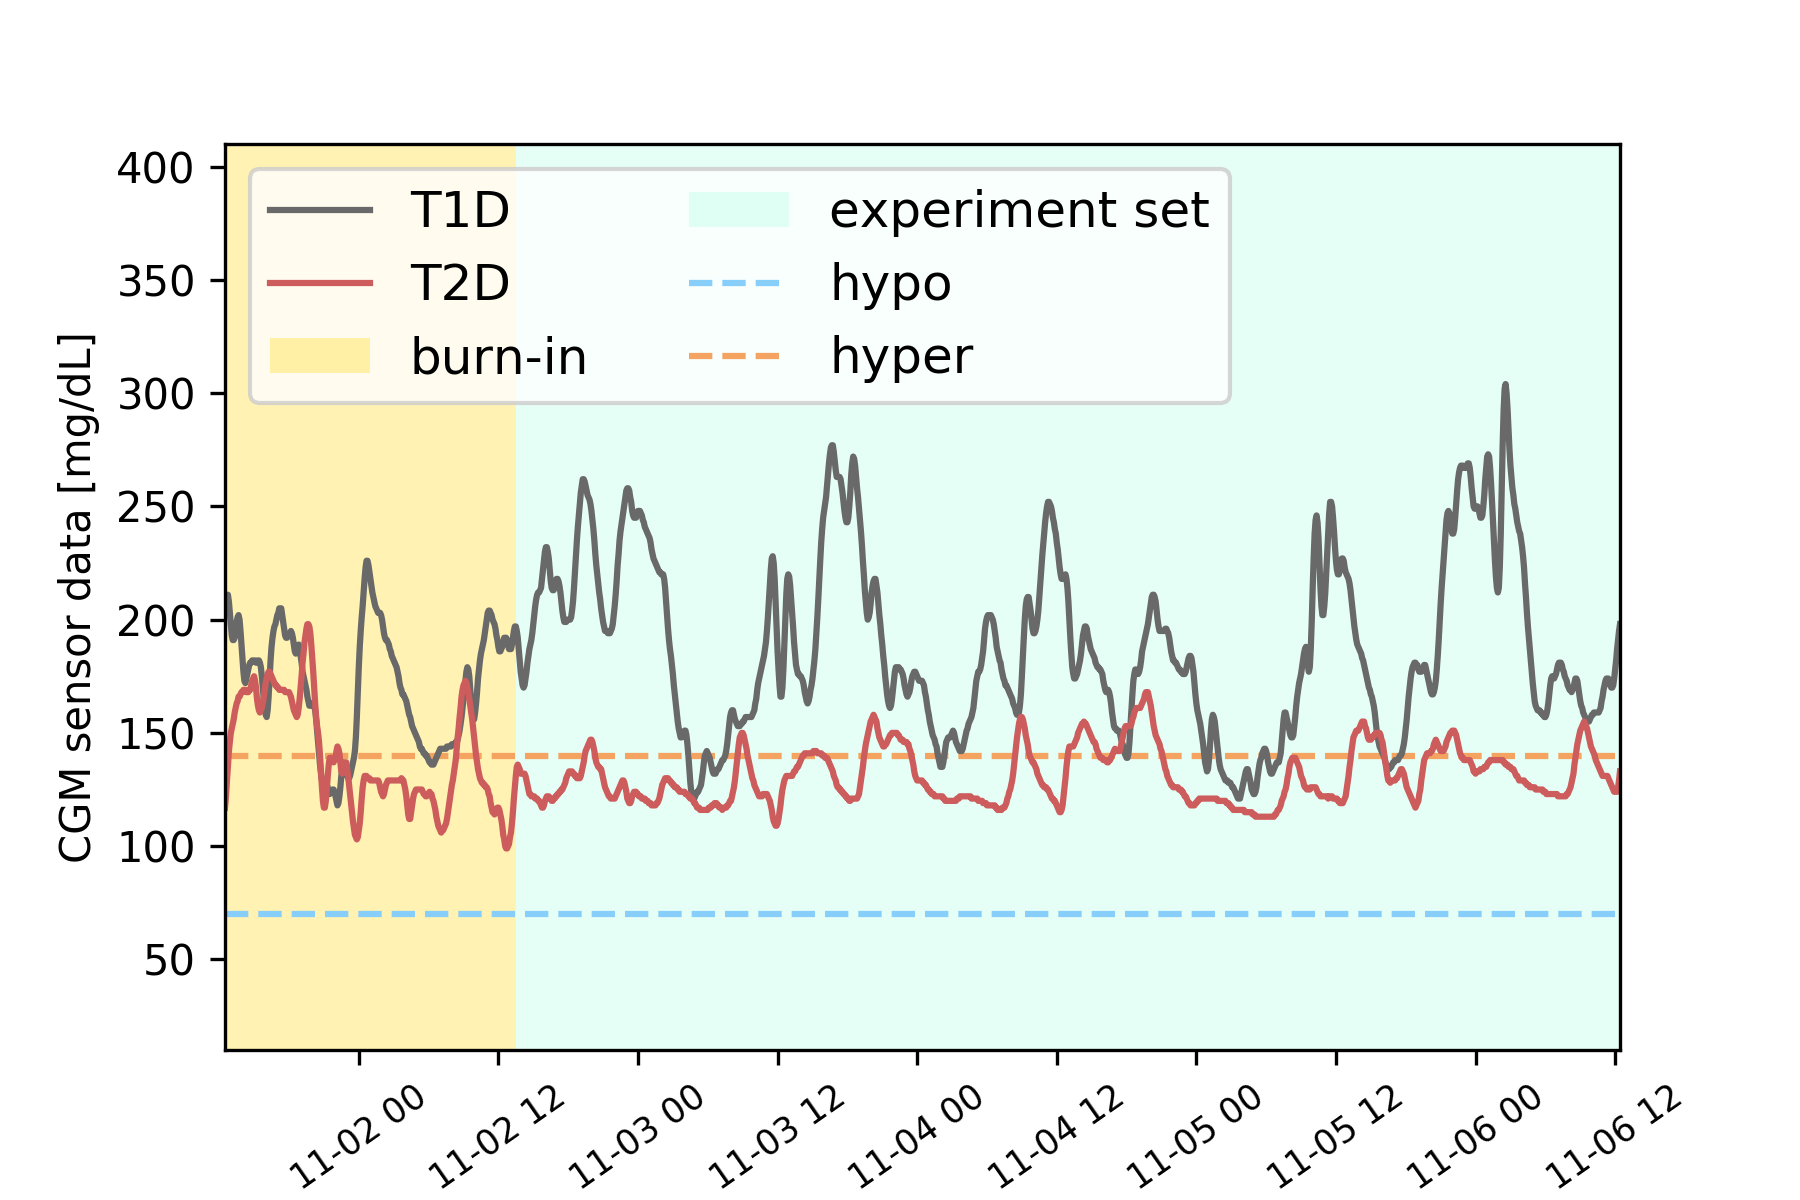
\includegraphics[width=0.8\textwidth]{part2/cgm_values.png}
\end{figure}

\section{CGM exploratory data analysis}
For each patient, the risk of hypo/hyperglycemia is determined by computing the Low Blood Glucose Index (\ac{LBGI}) and the High Blood Glucose Index (\ac{HBGI}), defined as in~\cite{fabris2016risk}.
LBGI and HBGI are summary statistics, extracted from a series of CGM data, that increases when the frequency and/or the extent of low CGM or high CGM readings increases.
These two indices are heavily influenced by the frequency and extent of hypo- and hyper-glycemic episodes.
To estimate LBGI and HBGI from CGM data we followed~\cite{kovatchev1997symmetrization}.
Figure \ref{fig:plots} shows the LBGI and HBGI distributions for T1D and T2D. The green areas at the bottom of each boxplot represents the low risk area for hypo/hyperglycaemia, as reported in literature~\cite{kovatchev1997symmetrization}.
As expected, the fraction of T1D patients experiencing risks of hyperglycaemia episodes is higher than T2D patients.

\begin{figure}[]
	\caption{Plots reporting the distributions of LBGI (left) and HBGI (right) for T1D and T2D. Green areas at the bottom of each plot represents low risk of hypo/hyperglycemia events.
		%  LBGI values below 2.5 indicate a low risk of hypoglycemia, while values above 5 correspond to an 
		%  Normal range for LBGI is $2.5-5$ and for HBGI is $10-15$.
	}\label{fig:plots}
	\centering
	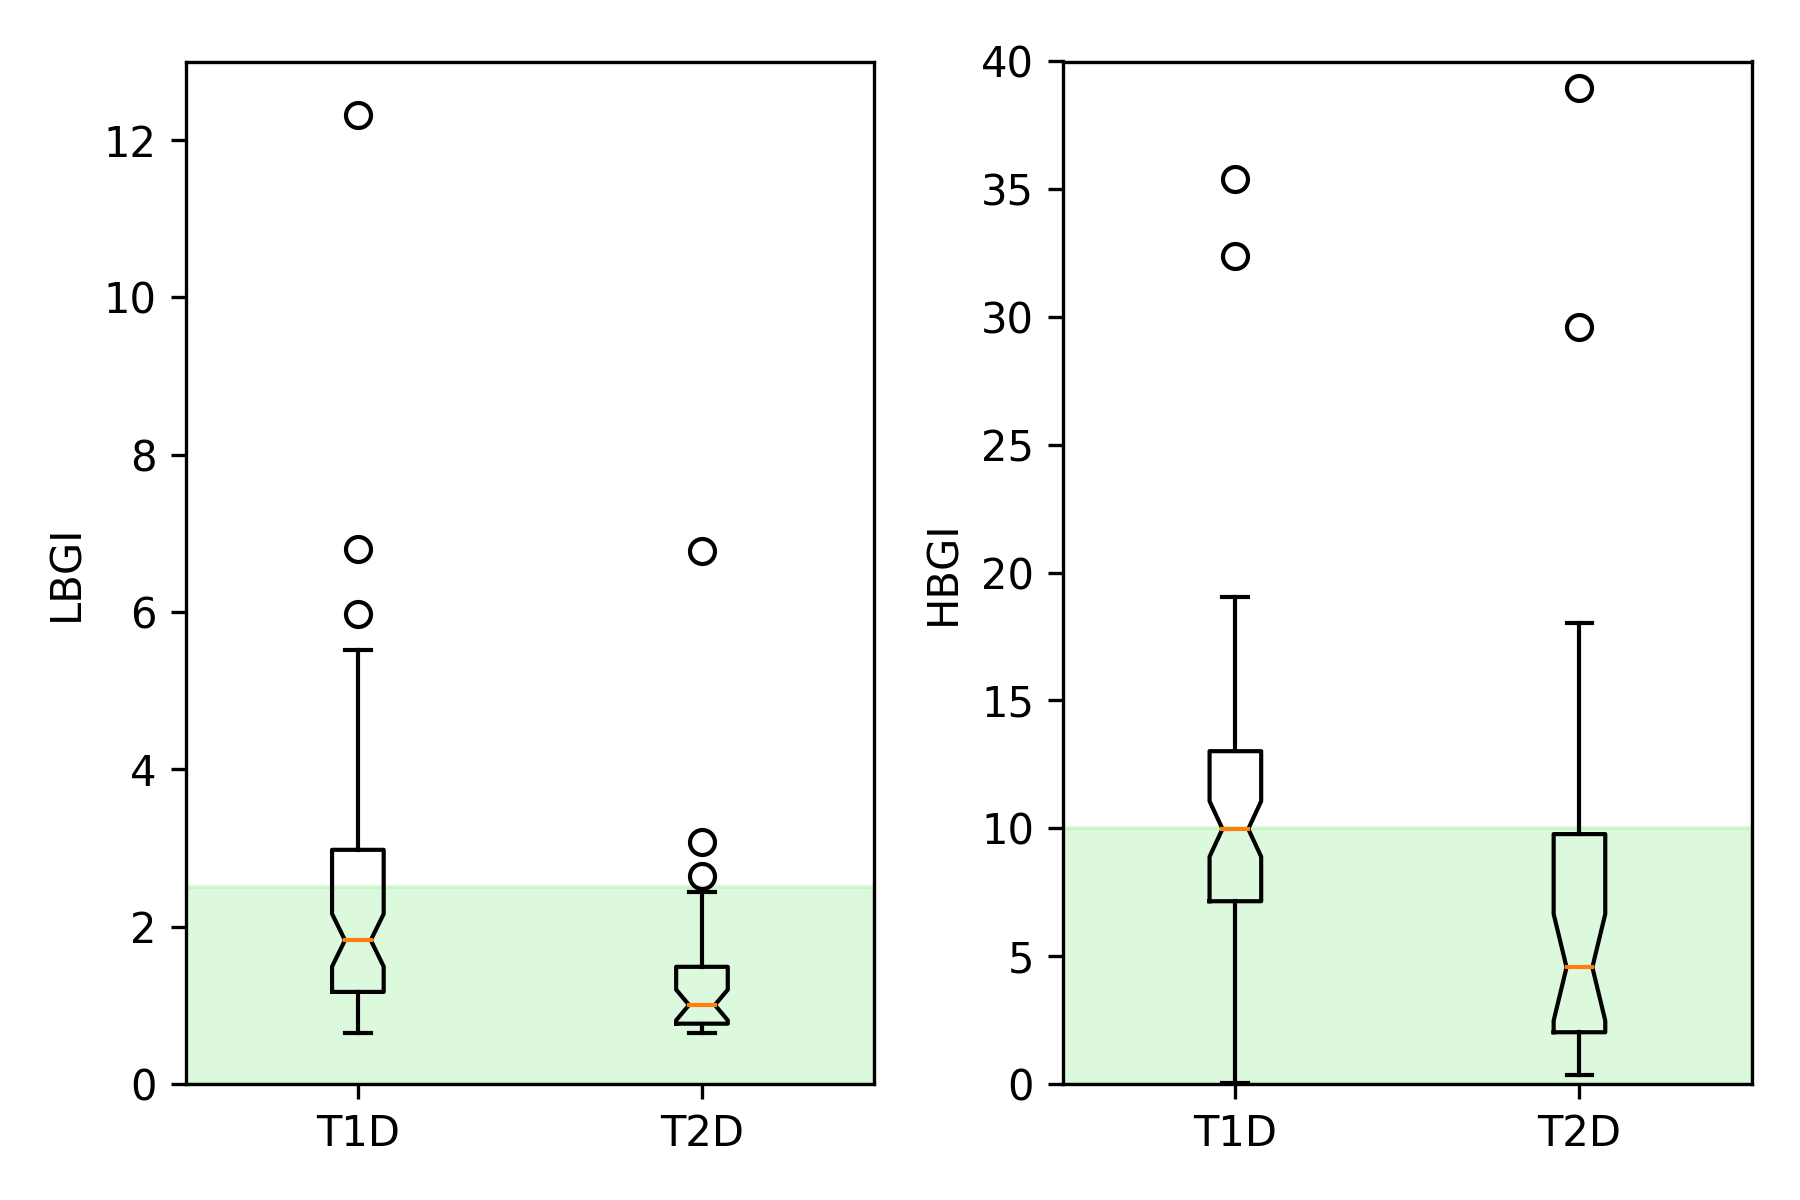
\includegraphics[width=0.8\textwidth]{part2/boxes.png}
\end{figure}

\section{Experimental design} \label{sec:diabete_expdesign}

Let's focus on the hyperparameters optimization strategy.
Given $y(t)$ for time points $t=1,\dots,T$, we split the time-series in two chunks: an initial {\em burn-in} of $T' = 300$ CGM observations and the {\em experiment set} made of the subsequent $T - T'$ samples (see Figure~\ref{fig:cgm}). For each model $\mathcal{M}_\mathcal{S}(\bm{\theta})$, and for each subject, we use the burn-in samples to optimize the hyperparameters $\bm{\theta}$ via grid-search cross-validation. In other words, the best hyperparameters $\bm{\theta}^*$  are chosen in order to minimize an index $J(\bm{\theta})$ estimated on cross-validation (CV) splits and defined differently according to the model. %, hence $\bm{\theta}^* = \argmin{\bm{\theta}} J(\bm{\theta})$.

In the context of time-series, the CV training split consists only of observations occurred before the corresponding validation samples; such CV flavor is sometimes referred to as {\em rolling forecasting origin}~\cite{tashman2000out}. The grid-search CV scheme promotes the identification of models capable of returning robust predictions. %, where the negative influence of the variable SNR is reduced.

Once the best hyperparameters $\bm{\theta}^*$ are identified, the model $\mathcal{M}_\mathcal{S}(\bm{\theta}^*)$ is fitted on the whole burn-in and it is used to perform online forecasting on the data points of the experiment set (\ie for $t = T'+1, \dots, T)$.

For each personalized model $\mathcal{M}_\mathcal{S}(\bm{\theta}^*)$ we calculate the accuracy for prediction horizons $\Delta T$ of $30, 60, \text{and}~90$ minutes. The performance is estimated by  RMSE and MAE, previously defined in Section~\ref{sec:performance_metrics}, that in the context of temporal forecasting, and assuming $n$ samples in the experiment set, can be rewritten as in Equation~\eqref{eq:forecasting_rmse} and~\eqref{eq:forecasting_mae}.

\begin{equation} \label{eq:forecasting_rmse}
\text{RMSE} = \sqrt{\frac{\sum_t(y(t+\Delta T) - \hat{y}(t+\Delta T))^2}{n}}
\end{equation}

\begin{equation} \label{eq:forecasting_mae}
\text{MAE} = \frac{\sum_t|y(t+\Delta T) - \hat{y}(t+\Delta T)|}{n}
\end{equation}

%for $t = T'+1,\dots,T-\Delta T$.
%\todo{non abbiamo mai detto quando vale la window size (36) come in sparacino2007}
We use $w=36$ as the size of the window in the moving-window paradigm and we  indicate with $\{\bm{x}_i, y_i\}_{i=1}^N$  the input/output pairs for machine learning model. 
%Machine learning models need to be trained on input/output pairs $\{\bm{x}_i, y_i\}_{i=1}^N$. In this work we employed a moving-window paradigm of size $w=36$. 
Therefore, each input $\bm{x}_i$ is a $w$-dimensional vector made of the CGM samples acquired at times $t=t_{i-w},\dots,t_i$, while the corresponding output $y_i$ is the CGM acquisition at time $t_{i+1}$.


\section{CGM forecasting results}
Taking into account the available information on treatments, we divided the dataset into four groups, namely T1D with microinfusion pump (32 subjects), T1D with insulin injection (40 subjects), T2D with rapid acting insulin (10 subjects) and T2D with other therapies (24 subjects).

For each group, we applied all forecasting models whose performance, expressed in term of MAE and RMSE, is presented in Table~\ref{tab:errors}. 
%obtaining predictions similar to the example in Figure~\ref{fig:fit}.
%Results are reported in Table~\ref{tab:errors}.
%\todo{The dataset was divided into two groups The subjects were divided in four groups, according to their diabetes type and the followed therapy.}
%A summary of the forecasting performance of the four methods, 
The forecasting errors clearly increase with the prediction horizon as the errors accumulate at each predicted time step.

KRR achieves the most accurate prediction overall and for almost every group of patients, although ARIMA results are comparable. Moreover, KRR loss of reliability from the first to the last prediction horizon is lower than for ARIMA.

Figure~\ref{fig:fit} displays an example of time-series forecast obtained with KRR showing the three different prediction errors at $30$, $60$ and $90$ minutes.

%    Only the samples in the left side of the plot are assumed to be available (green line).

\begin{figure}[tb]
	\caption{Online time-series forecasting obtained by KRR model. \textit{One-step-ahead prediction} (left): the green solid line shows the available samples; the dashed line represents one-step-ahead predictions that are obtained by applying the model on a moving window of 36 time-points. \textit{Open-loop forecast} (right): with passing time, the moving-window incorporates an increasing number of predicted points, accumulating errors; the dashed line represents forecast with a prediction horizon of 90'.
	Absolute prediction errors are evaluated with respect to future measures (red solid line).
		%  The dashed line in the left side of the plot In the right side of the plot we simulate an open-loop forecast where 
		%  Assuming that only the samples in the left side of the plot are available, the figure shows one-step-ahead predictions.
		%  On the right side, forecasts for a prediction horizon of 90 minutes are shown. 
		%  The absolute errors reported are expressed in $mg/dL$.
	}\label{fig:fit}
	\centering
	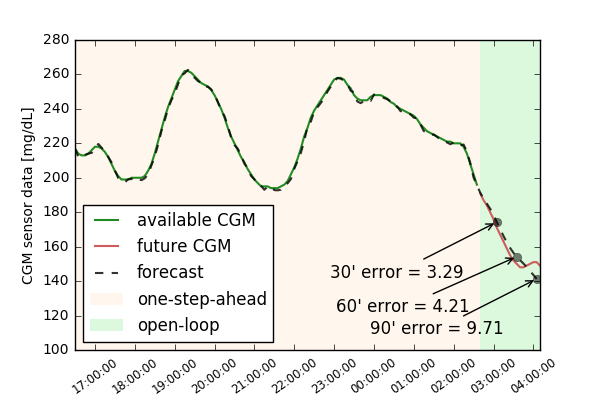
\includegraphics[width=0.8\textwidth]{part2/cgm_fit.png}
\end{figure}


\section{Conclusions and future works}

This chapter presented the last biomedical data science challenge of the Thesis.

We compared the performance of two types of data-driven strategies for online CGM forecasting: recursive filters and ML models. We also illustrate a general procedure for model personalization based on cross-validation with hyperparameters optimization via grid-search.

Finally, we showed that reliable CGM predictions can be obtained with ML models that do not need to recursively adjust their parameters along time.
%In the next future we plan to investigate further using more advanced methods comprising deep learning approaches with  and sparse regularization methods.

In the future, to improve the performance on long prediction horizon, we plan to investigate on sparse data representations with deeper architectures or regularized dictionary learning approaches.

\begin{table}[b!]
	\caption{Prediction errors $(\text{std})$ of the forecasting models for increasing prediction horizons overall and on the four groups. {\sl MP} = Microinfusion Pump, {\sl II} = Insulin Injection, {\sl RAI} = Rapid Acting Insulin, {\sl Other} = Other therapies. Bold numbers indicate best result.}
	\label{tab:errors}
		\begin{tabular}{lllllll}
			& \multicolumn{6}{c}{ARIMA}                                              \\ \cline{2-7}
			\multicolumn{1}{l|}{}                           & \multicolumn{3}{c|}{MAE mg/dL}          & \multicolumn{3}{c|}{RMSE mg/dL}         \\ \cline{2-7}
			\multicolumn{1}{l|}{}                           & 30 & 60 & \multicolumn{1}{l|}{90} & 30 & 60 & \multicolumn{1}{l|}{90}  \\ \hline
			\multicolumn{1}{l|}{Overall}                    & 11.5 (5.2) & 25.6 (12.5) & \multicolumn{1}{l|}{37.2 (20.3)} & 16.7 (7.9) & 37.1 (19.3) & \multicolumn{1}{l|}{53.8 (31.8)} \\
			\multicolumn{1}{l|}{T1D - {\sl MP}}   & 13.3 (3.6) & 30.3 (7.4) & \multicolumn{1}{l|}{45.3 (12.5)} & 19.5 (5.4) & 43.9 (10.9) & \multicolumn{1}{l|}{64.9 (18.1)}  \\
			\multicolumn{1}{l|}{T1D - {\sl II}}    & 13.4 (6.3) & 31.0 (16.2) & \multicolumn{1}{l|}{46.1 (27.1)} & 19.7 (10.6) & 45.1 (27.0) & \multicolumn{1}{l|}{66.6 (45.7)}  \\
			\multicolumn{1}{l|}{T2D - {\sl RAI}} & {\bf11.0 (3.3)} & {\bf 23.8 (6.5)} & \multicolumn{1}{l|}{33.2 (8.5)} & 16.2 (4.8) & 34.1 (8.3) & \multicolumn{1}{l|}{46.9 (10.9)}  \\
			\multicolumn{1}{l|}{T2D - {\sl Other}}      & 10.0 (5.1) & 21.4 (10.4) & \multicolumn{1}{l|}{29.2 (12.5)} & 13.6 (6.0) & 29.6 (12.7) & \multicolumn{1}{l|}{41.3 (16.5)}  \\ \hline
			
			\\
			& \multicolumn{6}{c}{KF}                                                \\ \cline{2-7}
			\multicolumn{1}{l|}{}                           & \multicolumn{3}{c|}{MAE mg/dL}          & \multicolumn{3}{c|}{RMSE mg/dL}         \\ \cline{2-7}
			\multicolumn{1}{l|}{}                           & 30 & 60 & \multicolumn{1}{l|}{90} & 30 & 60 & \multicolumn{1}{l|}{90} \\ \hline
			\multicolumn{1}{l|}{Overall}              & 46.8 (23.2) & 50.8(25.4) & \multicolumn{1}{l|}{159.6 (43.5)} & 58.3 (27.7) & 63.1 (30.3) & \multicolumn{1}{l|}{169.9 (47.1)} \\
			\multicolumn{1}{l|}{T1D - {\sl MP}}         & 56.6 (15.9) & 59.5 (15.2) & \multicolumn{1}{l|}{163.5 (26.7)} & 70.5 (19.0) & 74.3 (18.4) & \multicolumn{1}{l|}{177.5 (29.9)} \\
			\multicolumn{1}{l|}{T1D - {\sl II}}    & 59.9 (24.5) & 67.9 (26.7) & \multicolumn{1}{l|}{179.2 (38.9)} & 74.4 (28.7) & 83.5 (31.3) & \multicolumn{1}{l|}{193.8 (40.4)} \\
			\multicolumn{1}{l|}{T2D - {\sl RAI}} & 48.6 (20.4) & 50.9 (20.8) & \multicolumn{1}{l|}{195.2 (63.1)} & 60.4 (22.9) & 63.6 (24.1) & \multicolumn{1}{l|}{204.4 (63.8)} \\
			\multicolumn{1}{l|}{T2D - {\sl Other}}      & 33.0 (12.1) & 35.6 (15.8) & \multicolumn{1}{l|}{145.0 (30.4)} & 41.3 (14.2) & 44.3 (17.7) & \multicolumn{1}{l|}{150.1 (31.8)} \\ \hline
			
			
			\\
			
			& \multicolumn{6}{c}{KRR}       \\ \cline{2-7}
			\multicolumn{1}{l|}{}                           & \multicolumn{3}{c|}{MAE mg/dL}          & \multicolumn{3}{c|}{RMSE mg/dL} \\ \cline{2-7}
			\multicolumn{1}{l|}{}                           & 30 & 60 & \multicolumn{1}{l|}{90} & 30 & 60 & \multicolumn{1}{l|}{90}  \\ \hline
			\multicolumn{1}{l|}{Overall}                    & {\bf 11.1 (4.3)} & {\bf 25.1 (10.4)} & \multicolumn{1}{l|}{{\bf 35.2 (15.4)}} & {\bf 15.5 (6.7)} & {\bf 33.6 (13.8)} & \multicolumn{1}{l|}{{\bf 45.8 (19.7)}} \\
			\multicolumn{1}{l|}{T1D - {\sl MP}}   & {\bf12.9 (3.4)} & {\bf 30.2 (8.4)} & \multicolumn{1}{l|}{{\bf 43.1 (12.6)}} & {\bf17.9 (5.1)} & {\bf 40.2 (10.9)} & \multicolumn{1}{l|}{{\bf 56.0 (16.1)}}  \\
			\multicolumn{1}{l|}{T1D - {\sl II}}    & {\bf13.1 (4.9)} & {\bf 30.3 (10.6)}  & \multicolumn{1}{l|}{{\bf 43.1 (14.5)}} & {\bf18.6 (8.4)} & {\bf 40.5 (14.5)} & \multicolumn{1}{l|}{{\bf 55.8 (18.6)}}  \\
			\multicolumn{1}{l|}{T2D - {\sl RAI}} & 11.2 (2.9) & 24.1 (5.5) & \multicolumn{1}{l|}{{\bf 33.2 (7.1)}} & {\bf16.0 (4.7)} & {\bf 32.7 (7.5)} & \multicolumn{1}{l|}{{\bf 43.7 (9.5)}}  \\
			\multicolumn{1}{l|}{T2D - {\sl Other}}      & {\bf8.7 (2.3)} & {\bf 19.8 (6.9)} & \multicolumn{1}{l|}{{\bf 27.7 (11.8)}} & {\bf11.9 (3.4)} & {\bf 26.5 (8.9)} & \multicolumn{1}{l|}{{\bf 36.2 (14.4)}}  \\ \hline
			
			\\
			
			& \multicolumn{6}{c}{LSTM}                                              \\ \cline{2-7}
			\multicolumn{1}{l|}{}                           & \multicolumn{3}{c|}{MAE mg/dL}          & \multicolumn{3}{c|}{RMSE mg/dL}         \\ \cline{2-7}
			\multicolumn{1}{l|}{}                           & 30 & 60 & \multicolumn{1}{l|}{90} & 30 & 60 & \multicolumn{1}{l|}{90} \\ \hline
			\multicolumn{1}{l|}{Overall}                & 19.9 (10.6) & 44.0 (25.9) & \multicolumn{1}{l|}{61.3 (36.5)} & 26.2 (13.4) & 55.0 (30.0) & \multicolumn{1}{l|}{74.7 (41.3)} \\
			\multicolumn{1}{l|}{T1D -{\sl  MP}}   & 22.9 (9.1) & 51.6 (21.5) & \multicolumn{1}{l|}{71.6 (27.0)} & 30.6 (11.6) & 65.7 (27.0) & \multicolumn{1}{l|}{89.8 (33.5)} \\
			\multicolumn{1}{l|}{T1D - {\sl II}}    & 24.5 (12.9) & 56.5 (33.1) & \multicolumn{1}{l|}{81.4 (45.8)} & 31.2 (14.9) & 68.8 (35.9) & \multicolumn{1}{l|}{97.0 (48.4)} \\
			\multicolumn{1}{l|}{T2D - {\sl RAI}} & 18.3 (6.7) & 39.4 (14.8) & \multicolumn{1}{l|}{54.1 (21.0)} & 25.7 (10.1) & 51.6 (21.7) & \multicolumn{1}{l|}{67.7 (29.1)} \\
			\multicolumn{1}{l|}{T2D - {\sl Other}}      & 16.8 (8.9) & 35.0 (17.7) & \multicolumn{1}{l|}{47.0 (26.5)} & 22.2 (12.1) & 43.4 (19.0) & \multicolumn{1}{l|}{56.5 (27.3)} \\ 
			
			\hline
			
		\end{tabular}
\end{table}
